\chapter{Wstęp}

\section{Cel zajęć}
Celem niniejszej pracy była analiza oraz dobór parametrów systemu adaptacyjnego w zależności od występujących w systemie zakłóceń oraz transmitancji obiektu, którym sterowano. Przyjęty model przedstawiono na rysunku \ref{model_systemu}.

\begin{figure}[h!]
	\centering
	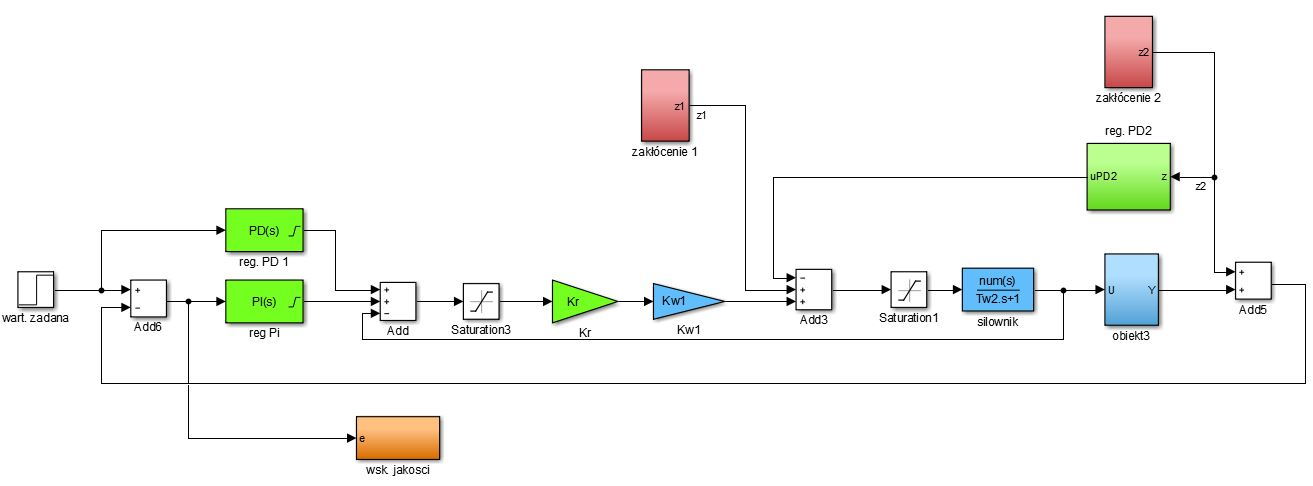
\includegraphics[scale = 0.5]{fig/model_systemu.jpg}
	\caption		
	{Model układu sterowania}
	\label{model_systemu}
\end{figure} 

\section{Model obiektu}
Obiekt sterowania jest modelem Strejca, opisany transmitancją \ref{model_systemu}. Wzór ten ze względu na swoją postać - \textit{n} szeregowo połączonych obiektów inercyjnych pierwszego rzędu z dodatkowym opó\'znieniem czasowym, może opisywać dynamikę np. instalacji kaskadowo połączonych zbiorników.W zależności od dynamiki układu, współczynnik \textit{n} może przyjmować coraz to większe wartość $1, 2, 3, ...$. Na potrzeby niniejszej pracy ograniczono się do rozpatrywania omawianego modelu rzędu pierwszego, drugiego oraz trzeciego. 
\begin{equation}\label{main_trans}
G(s) = \dfrac{K_0}{(T_0 \cdot s + 1)^n} \cdot e^{-\tau \cdot s} 
\end{equation}
Przyjęto następujące wartości parametrów: \\
$K_0 = 10$,\\
$T_0 = 1$,\\
$\tau = 1$.\\
 Przedstawione na rysunku \ref{model_systemu} bloczki \textit{Kr}, \textit{Kw1} i \textit{siłownik} opisują dynamikę urządzenia wykonawczego, którym w tym przypadku mógłby być np. zawór regulujący przepływ cieczy. Siłownik opisany jest transmitancją \ref{silownik}
\begin{equation}\label{silownik}
G_s(s) = \dfrac{Kw2}{Tw2 \cdot s + 1}
\end{equation}
gdzie: \\
$Tw2 = 0.1$, \\
$Kw2 = 5$. \\
%


\section{Regulatory}
Poszczególne regulatory znajdujące się na schemacie \ref{model_systemu} opisano następującymi wzorami: 
\begin{equation}\label{reg1}
PD_1 = P1+D1 \cdot s
\end{equation}
\begin{equation}\label{reg2}
PD_2 = P2+D2 \cdot s
\end{equation}
\begin{equation}\label{reg3}
PI = P3 + \dfrac{I3}{s}
\end{equation}

Regulatory $PD_1$ i $PD_2$ to regulatory proporcjonalno-różniczkujące o wzmocnieniach $\alpha_1$ i $\alpha_2$ oraz czasach różniczkowania $\beta_1$ i $\beta_2$. Regulator $PI$ to regulator proporcjonalno-całkujący o wzmocnieniu $\gamma$ i współczynniku całkowania $\delta$. \\
Sygnał sterujący generowany jest głównie przez układ dwóch równolegle połączonych regulatorów  $PI$ i $PD_1$. Pierwszy z nich działa w klasycznej pętli regulacji z ujemnym sprzężeniem zwrotnym. Głównym zadaniem regulatora $PI$, oprócz stabilizacji sygnału wyjściowego na zadanym poziomie, jest niwelowanie uchybu ustalonego. Drugi regulator - $PD_1$, działa w pętli \textit{feedforward} reagując na zmiany wartości zadanej. Dzięki zastosowaniu tego rozwiązania osiągnięto lepszą dynamikę układu regulatorów, niż w przypadku pojedynczego regulatora $PI$, zachowując jednocześnie   eliminacje uchybu ustalonego. \\
W celu zabezpieczenia układu przed niepożądanym działaniem zakłóceń wprowadzono dwie dodatkowe modyfikacje. Pierwsza z nich, to dodatkowa pętla sprzężenia tworząca zamknięty układ w obrębie urządzenia wykonawczego. Ma ona za zadanie wraz ze wzmocnieniem proporcjonalnym $Kr$, niwelować wpływ zakłócenia $z_1$ na sygnał sterujący podawany na obiekt.  Drugim zabezpieczeniem jest regulator $PD_2$ pracujący w pętli \textit{feedforward} od zakłócenia $z_2$. Zadaniem tego regulatora jest przeciwdziałanie zakłóceniu podawanemu bezpośrednio na sygnał wyjściowy z obiektu.

\section{Filtr wind-up}
Jak można zauważyć na rysunku \ref{model_systemu} do modelu obiektu wprowadzono ograniczenia na wartość sygnału sterującego w postaci saturacji. Ma to na celu odwzorowanie rzeczywistej sytuacji gdy sygnał sterujący jest ograniczony np. przez minimalne i maksymalne napięcie podawane na urządzenie wykonawcze. Sytuacja ta negatywnie wpływa na jakość regulacji, co zauważono w przypadku działania regulatora $PI$, który bardzo szybko się nasycał - generował sterowanie o wartościach minimalnych lub maksymalnych. Wiązało się to z nadmiernym wzrostem członu całkującego, szczególnie dla obiektu drugiego i trzeciego rzędu. Aby temu zapobiec wprowadzono w strukturze regulatora filtr typu wind-up, który działał na zasadzie wstecznej korekcji wartości całki. Schemat tak zmodyfikowanego regulatora znajduje się na rysunku \ref{windUp}. Przyjęto, że współczynnik $K_b$ będzie miał wartość $\frac{1}{sqrt(\delta)}$.

\begin{figure}[h!]
	\centering
	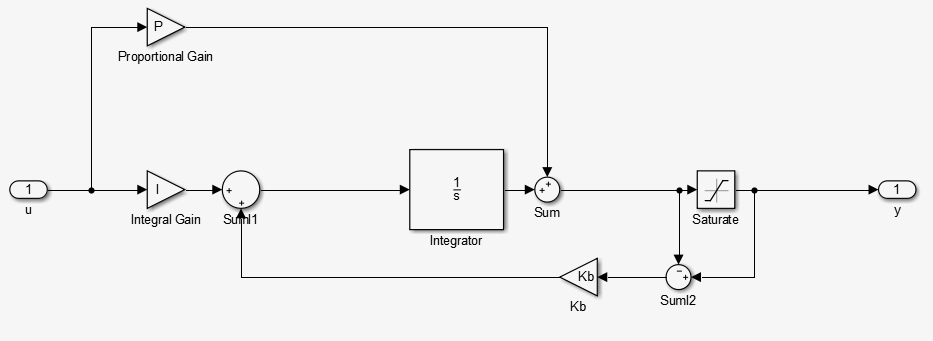
\includegraphics[scale = 0.6]{fig/windUp.jpg}
	\caption		
	{Regulator PI z filtrem wind-up.}
	\label{windUp}
\end{figure} 

\section{Wska\'znik jakości}
W ramach projektu należało przeprowadzić optymalizację poszczególnych parametrów podanych powyżej regulatorów, tj. $P1$, $D1$, $P2$, $D2$, $P3$, $I3$. Wskaźnikiem jakości, na mocy którego optymalizowano działanie całego układu, była całka z modułu uchybu:
\begin{equation}\label{wsk_jak}
J = \int |e(t)| dt
\end{equation}
gdzie: \\
$e(t) = r(t) - y(t)$ - uchyb regulacji.\\ 

 Ponadto, przyjęto iż oczekiwanym efektem optymalizacji będzie takie zachowanie układu, by bez względu na wartości zakłóceń $z_1$ i $z_2$, efekt stabilizacji był jak najlepszy w sensie przyjętego wska\'znika jakości \ref{wsk_jak}.

